\documentclass[tikz]{standalone}
\usepackage{tikz}
\usetikzlibrary{positioning, graphs}
\usetikzlibrary{graphs.standard}
\begin{document}
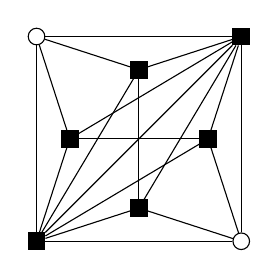
\begin{tikzpicture}
    [circle_node/.style={circle, draw, inner sep = 0, minimum size = 0.6em},
     rectangle_node/.style={rectangle, draw, inner sep = 0, minimum size = 0.6em, fill=black}]

    \graph[clockwise, radius = 2.5em, phase = 0, empty nodes,
        nodes=rectangle_node]{subgraph I_n[n = 4, name = A]};

    \node[rectangle_node]  (a) at (1.3, 1.3) {};  
    \node[rectangle_node]  (b) at (-1.3, -1.3) {};  
    \node[circle_node]  (c) at (1.3, -1.3) {};  
    \node[circle_node]  (d) at (-1.3, 1.3) {};  

    \draw (a) -- (c) -- (b) -- (d) -- (a);
    \draw (a) -- (b);
    \draw (A 1) -- (A 3);
    \draw (A 2) -- (A 4);
    \draw (A 1) -- (c) -- (A 2);
    \draw (A 3) -- (d) -- (A 4);
    \foreach \i in {1, 2, 3, 4}{
        \draw (a) -- (A \i);
        \draw (b) -- (A \i);
    }
\end{tikzpicture}
\end{document}